\section{Jackson Kennedy}

\subsection{IOS App}
As a big part of the project, I took on the IOS portion of the project as my own task.
\\\\
Pictured below is the main screen where the user will lock/unlock the smartLock. The phone screen you see is not a simple concept drawing, but is actually coded. The buttons both work, and reflect the lock status in the database. Attached is a picture of the database reflecting the status, 1 - unlocked, 0 - locked. This is significant because now, data can be pulled from the cloud in real time.
\begin{figure}[h]
     \centering
     \begin{subfigure}{0.3\textwidth}
         \centering
         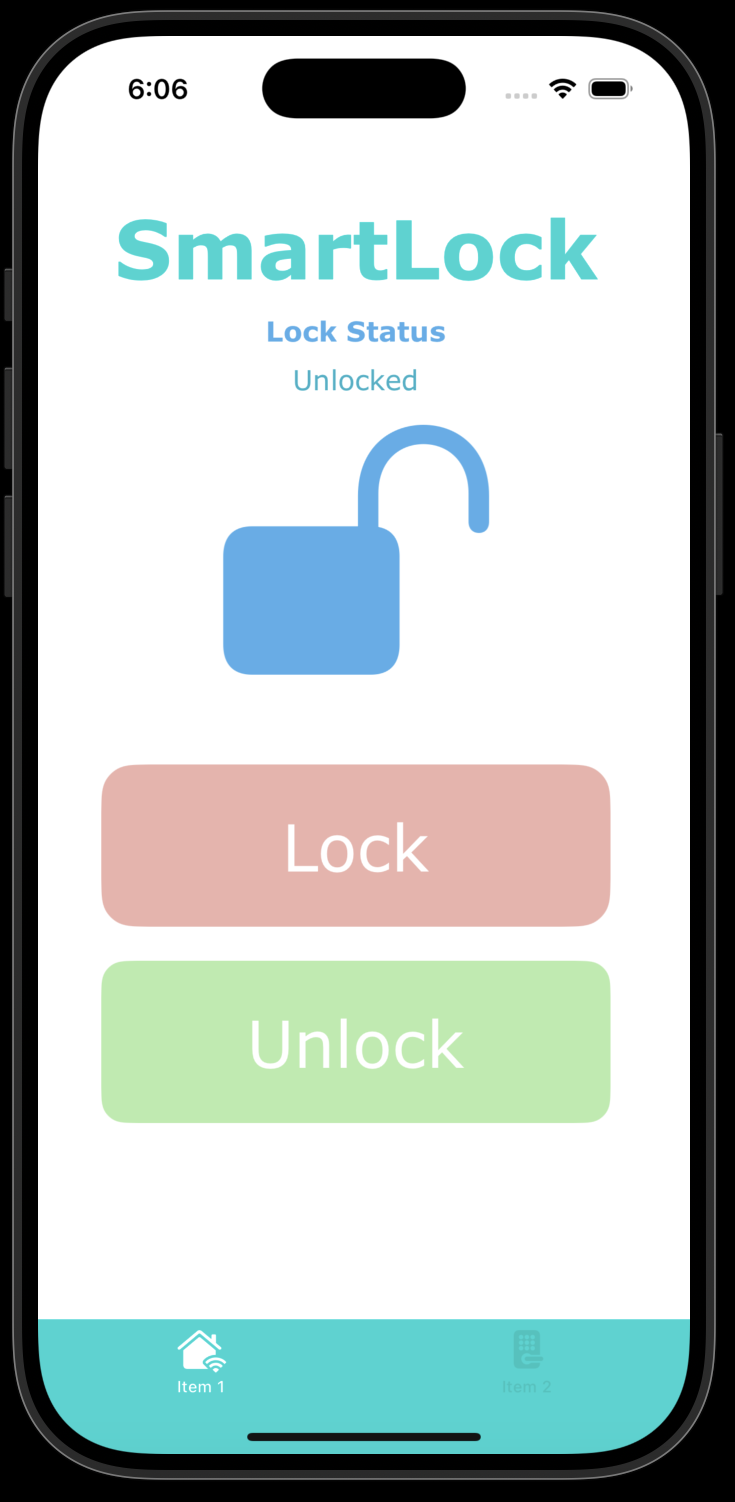
\includegraphics[width=\linewidth]{./img/unlockedPage.png}
         \caption{}
         \label{fig:1a}
     \end{subfigure}
     \begin{subfigure}{0.6\textwidth}
         \centering
         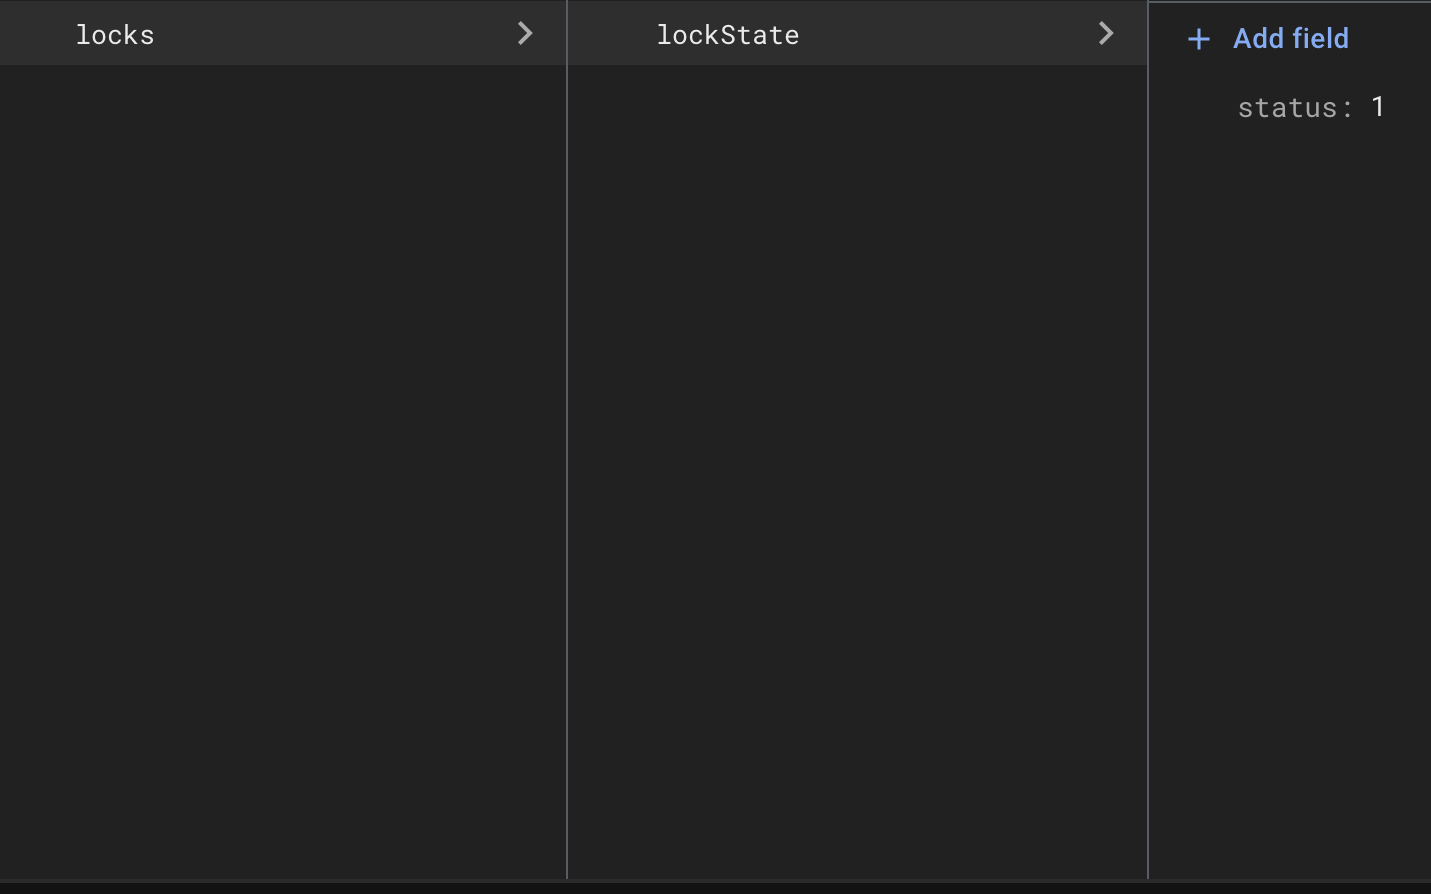
\includegraphics[width=\linewidth]{./img/lockState.png}
         \caption{}
         \label{fig:1b}
     \end{subfigure}
     \caption{Unlocked State on mobile device reflecting in cloud database.}
     \label{fig:1}
\end{figure}
\newpage
Additionally, I have set up the framework and programmed another screen that is accessible via the toolbar on the bottom of the screenshot. This is not yet connected to any database, but I populated it with a sample array of sample pins that I will later set up for secure user generation. This sets up the app for easy configuration down the line, where user generated pins can be used to populate the array and present as a part of a scrollable view on the app to consolidate the user's data.

\begin{figure}[htbp]
    \centering
    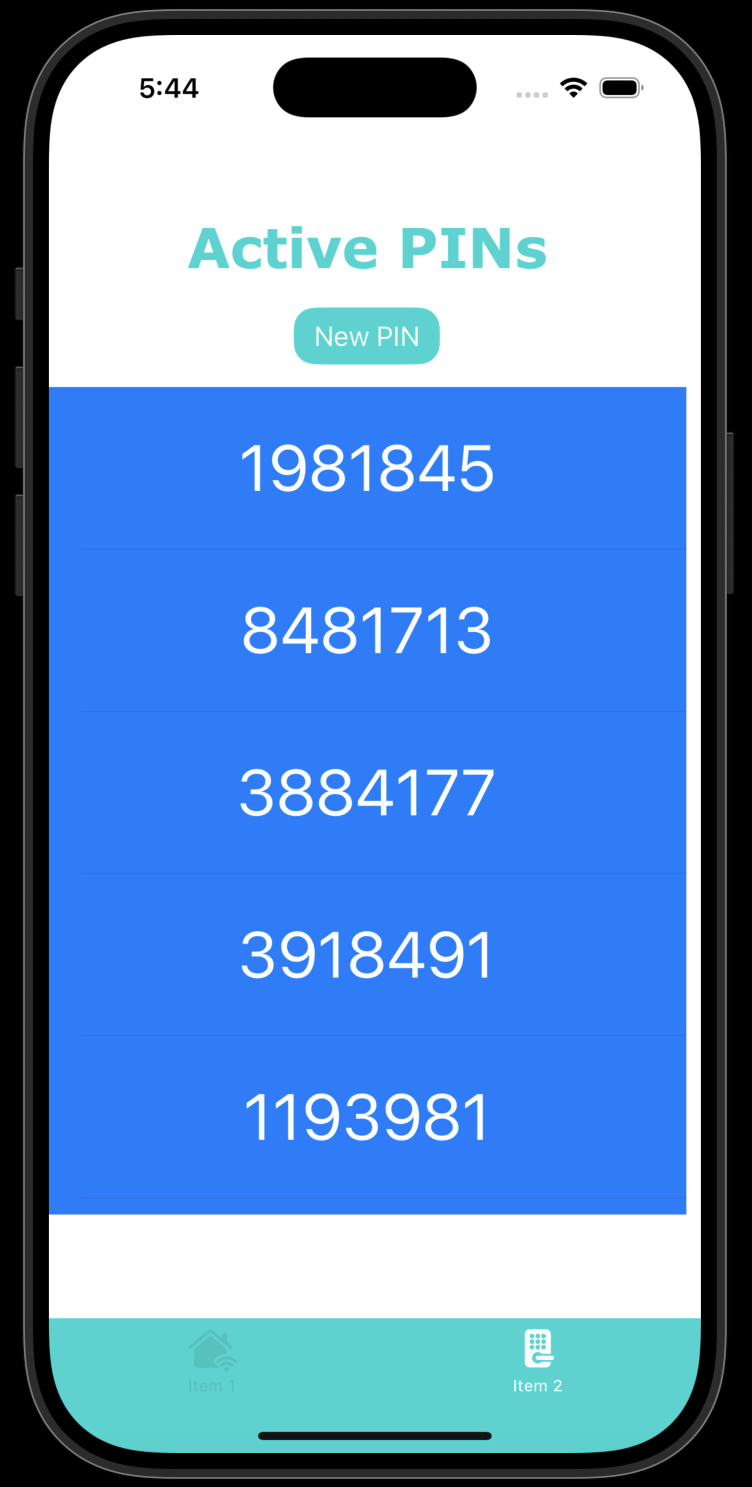
\includegraphics[width=0.4 \linewidth]{./img/pinPage.png}
    \caption{Pin Tab}
    \label{fig:pin}
\end{figure}
One of the main requirements for the end of this quarter was to get the phone communicating with the cloud, which I have been successful in transmitting data from the IOS device to the cloud provider and database.

\subsection{Test Plan}

On top of the mobile app, I helped to contribute to the test plan by writing a lot of the test plan based on project requirements. This includes things like hardware testing, and software communication testing.

\subsection{Morphological Chart}

I completed my section in the Morphological chart and added my design ideas and communication protocols.

\subsection{Mind Maps}

I helped to create the mind map by adding relevant sections and subsections with related technologies and ideas. This mind map helped us to push forward to strategize our different sections and account for different features and fields involved in the project.